%%%%%%%%%%%%%%%%%%%%%%%%%%%%
% Literature Review for Glaciology class
% Fall 2015
% Snow distribution on glaciers
%%%%%%%%%%%%%%%%%%%%%%%%%%%%

\documentclass[12pt]{article}
\usepackage[letterpaper, margin=1in]{geometry}
\usepackage{graphicx}
\usepackage{natbib}
\usepackage{wrapfig}

\begin{document}

\title{Snow distribution on glaciers}
\author{Alexandra Pulwicki \\ Earth Science SFU}
\date{\today}
\maketitle

\begin{abstract}
Glacier mass balance input is controlled mainly by the distribution of snow. The spatial variability of accumulation in alpine regions therefore has major impacts on mass balance. Processes such as orographic lifting, preferential deposition, and wind redistribution, all arising from the interaction of atmospheric conditions and steep topographic gradients, strongly affect the distribution of snow. Dynamic and statistical models have been used to relate meteorological and topographic variables to snow accumulation in order to better understand the effects of these processes. These models rely on accurate measurement of snow distribution, so a number of different methods have been employed. Snow probing, ground penetrating radar, and digital elevation model subtraction are widely used accumulation measurement methods that vary considerably in their spatial resolution, cost, and ease of use. Snow distribution on glaciers has not been studied extensively and model and measurement method application to this topic is still sparse. Results from previous studies have shown large spatial variability, at many scales, in snow accumulation and a dependence on multiple processes that affect snow distribution. Accumulation in the St. Elias Mountains is particularly poorly understood, largely because the glaciers are remote and difficult to access. There is therefore a need to understand snow accumulation in this region and how it varies both between glaciers and within glacierized basins. 

\end{abstract}
\pagebreak

\tableofcontents
\pagebreak

\section{Introduction}
Snow accumulation, as the dominant input of mass to alpine glaciers, plays an important role in governing their mass balance and the hydrology of alpine catchments more broadly. This has implications not only for the availability of water for local ecological and anthropogenic uses \citep{ONeel2014,Barnett2005}, but also for rates of global sea-level rise \citep{Gardner2013}. It is therefore critical to thoroughly understand the spatial distribution of snow on glaciers. Achieving such an understanding however is complicated by the fact that snow distribution in alpine regions is not uniform or static, but rather highly variable and influenced by diverse and dynamic processes operating on multiple spatial and temporal scales. Although previous research has attempted to account for these processes through the development of various techniques of measurement and modelling, little is known about how they operate in glacialized alpine environments. This severely limits possibilities of quantifying and predicting snow distribution on glaciers, particularly in remote locations where frequent empirical measurements are difficult \citep{Nolan2015}.

This literature review examines what is currently known and unknown about the topic of snow accumulation on glaciers and its spatial variability. The following section begins with an overview of accumulation variability within alpine regions in general, as there is a considerably greater breadth of studies devoted to snow in non-glacierized alpine basins. Section 3 reviews different ways of modelling the distribution of snow in alpine environments, while Section 4 describes methods for measuring accumulation and their relative merits and challenges. Section 5 compiles studies that specifically look at accumulation variability on glaciers and summarizes their key findings. The final section focuses on the St. Elias Mountains, a large glacierized region where little is known about snow distribution and its effects on glacier mass balance.

\section{Accumulation variability}
The spatial distribution of snow accumulation can vary significantly. This is a result of interactions between spatially and temporally variable atmospheric conditions and heterogeneous topography \citep{Deems2006, Liston2006}. Understanding and predicting snow distribution therefore requires accounting for factors that include atmospheric circulation, precipitable water, air pressure, air temperature, wind speed and direction, elevation, slope exposure, presence of orographic barriers, surface slope and aspect, surface roughness, and relief \citep{McGrath2015}.

\subsection{Topographic scales}
Snow accumulation is spatially variable on point scales ($<$5 m), hillslope scales (1--100 m), watershed scales (100--10,000 m) and regional scales (10--1000 km) \citep{Clark2011}. The features and conditions that lead to variability at these scales differ (see Table \ref{scale}) and their relative importance depends on the topography and climate of the study area. Inclusion of parameters that describe relevant processes at multiple scales has been shown to improve models that aim to explain measured snow distribution \citep{Marchand2005, Clark2011}. 

Point-scale variability is generally associated with surface roughness effects and the presence of small obstacles. These effects can be significant in vegetated landscapes or when the surface is very rough (e.g. boulder field). Many parts of a glacier though are characterized by a relatively smooth surface, with roughness lengths on the order of centimeters \citep{Hock2005}. In these areas, point-scale variability of snow is low. However, in heavily crevassed regions, point-scale variability can be large and thus exert a dominant control on snow distribution in the area \cite{McGrath2015}. 

Hillslope-scale variability is caused by variations in the surface topography of the glacier. The curvature and slope of the surface as well as the presence of local ridges or depressions can affect where snow is located \citep{Bloeschl1999, Sold2013}. Avalanching can also redistribute snow, especially on the margins of a glacier \citep{Bloschl1991, Mott2008}. 

Watershed-scale variability results mainly from the effects of changing elevation and aspect on atmopsheric conditions \citep{Clark2011}. In particular, orographic lifting and shading can result in higher elevation and north-facing areas of the glacier having more snow than other areas \citep{Mott2008, Sold2013}. Gradients in temperature from elevation changes also affect the freezing level, which determines whether precipitation falls as snow or rain \citep{Bloschl1991}. For example, \cite{Machguth2006} found a strong influence of elevation in determining accumulation on Findel Glacier in Switzerland.

Regional variability occurs when areas within a mountain range have differing amount of snow. Often, this results from horizontal precipitation gradients and rain shadows forming on the lee side of topographic divides. Areas with large, steep mountains are especially affected by these processes.

Generally, spatial variability increases with spatial scale \citep{Clark2011}. Extent and spacing of measurements must therefore capturing variability both across the study area and at smaller scales. \cite{Clark2011} notes that studies of snow water equivalent (SWE) that have been conducted in alpine environments vary considerably in the extent and spacing of their measurements. 

\begin{table}[]
\centering
\caption{Relevant spatial scales for snow variability on glaciers. Information from \cite{Clark2011}.}
\label{scale}
\begin{tabular}{lll}
\textbf{Scale} & \textbf{Length} & \textbf{Associated glacier feature}                     \\ \hline
Point          & $<$5 m         & Crevasses                                               \\
Hillslope      & 1--100 m        & Local surface topography (curvature, slope), avalanching        \\
Watershed      & 100--10,000 m   & Elevation, aspect                                       \\
Regional       & 10--1000 km     & Horizontal precipitation gradient across mountain range
\end{tabular}
\end{table}

\subsection{Snow drift and preferential deposition}
Snow drift and preferential deposition are crucial factors that influence the distribution of snow \citep{Lehning2008, Winstral2002, Clark2011}. Sharp changes in topography cause convergent and divergent airflows close to the surface, leading to turbulence and vorticity. This modifies mean wind (and snow particle) velocities, and thus can influence snow distribution via snow drift and/or preferential deposition \citep{Mott2008, Lehning2008, Dadic2010}.

Snow drift is the erosion and deposition of already deposited snow \citep{Dadic2010}. In general, erosion on the windward side is caused by increased wind speeds and deposition on the lee side of ridges is due to decreased wind speeds \citep{Liston1998, Mott2008, Dadic2010}. 

Preferential deposition is inhomogeneous precipitation in the absence of local erosion \citep{Lehning2008}. It is mainly governed by winds, where higher wind velocities and updrafts on the windward side of ridges cause reduced deposition while reduced wind velocities on the lee side enhance deposition. This process can occur at relatively low wind speeds because it does not require the lifting of already deposited snow  --- instead, it only needs to act with or against the falling snow \citep{Mott2008, Dadic2010}. 

Both processes described can occur at multiple spatial scales. Enhanced accumulation has been observed on the point-scale in small depressions and on lee sides of obstacles, on the hillslope scale on the lee side of ridges, and at the watershed scale on sheltered aspects \citep{Harrison1986, Bloeschl1992, Mott2008, Winstral2002, Clark2011}. 

\section{Snow distribution models}
The distribution and variability of a parameter, such as snow, can be estimated using either dynamic or statistical models. These models help to determine relevant processes that affect the distribution of snow, generally by relating its distribution to meteorological and topographic descriptors or conditions. Inferences made from these models drive the direction of future studies and provide valuable insight into understanding why variability arises.  

\subsection{Dynamic models}
Deposition and redistribution of snow can be represented using physically based, spatially distributed models. The general aim of these models is to simulate surface processes and how they vary spatially and temporally \citep{Mott2008}. These models usually consider atmospheric conditions including freezing level, precipitation rates, relative humidity, and wind speed and direction; as well as processes such as orographic lifting, cloud formation, downslope evaporation, advection and fallout, snow metamorphism, and wind redistribution of snow (erosion, saltation) due to terrain induced turbulence \citep{Smith2004, Liston2006, Lehning2008, Mott2008}.  Modelling the dynamically induced flows of these components together describes the preferential deposition and redistribution of snow in alpine environments \citep{Lehning2008,Mott2008,Dadic2010}.

Many models have been developed to describe preferential deposition and redistribution. Early models were developed for flat or gently rolling terrain where boundary layer flow is better understood \citep{Dadic2010}. Boundary layer flow in steep terrain is generally non-linear though \citep{Mott2008, Dadic2010}, so a number of different approaches have been applied.  For example, \cite{Dadic2010} and \citep{Lehning2008} solved non-hydrostatic, compressible Navier-Stokes equations in 3-D and aimed to conserve momentum, heat, mass, and states of water, to model wind flow velocities. \cite{Smith2004} employed Fourier transforms in a linear orographic model, which allowed for the more accurate representation of complex terrain. 

Dynamic models are a valuable way to determine accumulation variability. Since they use physically consistent processes, they can be applied to any site and generate values for each grid cell. They can also be used in different climatic conditions, allowing for predictions of accumulation change \citep{Clark2011}. Furthermore, a historic data set of variables is not needed to generate a meaningful output. Another advantage of dynamic models is that they allow for high temporal resolution (e.g. \cite{Mott2008} has a 1 hour time step), which allows for snowpack evolution to be examined.

Application of dynamic models is however operationally complex and computationally expensive, and also requires a diverse set of observations. Input parameters usually include temporally varying values for precipitation, wind speed and direction, air temperature, and relative humidity \citep{Liston2006}. Although these parameters can be obtained from meteorological stations, spatially distributed values --- found using atmospheric models --- are also required \citep{Liston2006, Mott2008}. For example, \cite{Dadic2010} used meteorological data from three automatic weather stations located throughout the study basin, while in the study done by \cite{Mott2008} monthly stake measurements were needed. Such a well-monitored basin can be difficult to achieve in remote or inaccessible areas. A number of other dynamic models --- such as those described in \cite{Fowler2007} --- use global circulation model (GCM) values to drive local circulation models, but it was shown that model output strongly depended on GCM boundary choice.  Even with sufficient and appropriate input data, the models must assume a number of parameters and simplify parameter relationships (e.g. constant mean wind speed \citep{Mott2008}) to characterize the atmosphere, which may not realistically describe conditions. Additionally, the models do not account for all modes of snow transport. For example, snow deposition due to avalanching can be an important process of snow transport that is not captured in current models \citep{Mott2008}. 

\subsection{Statistical models}

Statistical models of snow variability establish empirical relationships between snow distribution and external variables \citep{Fowler2007}. This method assumes that local distribution is forced by external factors, such a meteorological conditions or topography.

\subsubsection{Statistical downscaling}

Statistical downscaling is the process of determining an empirical relationship between large-scale atmospheric conditions and regional climates \citep{Fowler2007}. In general, this relationship is expressed as a function $F$ such that regional variables $R$ are found by $R=F(X)$ where $X$ encompasses large-scale climate variables \citep{Fowler2007}. These models are trained and validated using gridded reanalysis data from GCMs ($X$) and point observations ($R$). Performance of these models is measured using correlation coefficients, distance measures (e.g. root mean squared error), or explained variance \citep{Fowler2007}. 

There are three main types of statistical models \citep{Fowler2007}. The first is a regression model, which directly quantifies a relationship between a local variable and a number of large-scale variables. Statistical methods such as multiple linear regressions \citep{Hanssen-Bauer1998}, principal component analysis \citep{Kidson1998}, canonical-correlation analysis \citep{Busuioc2001}, neural networks \citep{Zorita1999}, and singular value decomposition \citep{Widmann2003} can be employed.  The second type of model is a weather typing scheme, which relates the occurrence of a particular `weather class' to local variables. Weather classes can be found using empirical orthogonal functions or cluster analysis \citep{Fowler2007}. The third model uses weather generators that simulate local precipitation occurrences with a chosen distribution of precipitation amount \citep{Fowler2007}. The large-scale input variables that are usually chosen (e.g. sea-level pressure, geopotential heights) for statistical downscaling are representative of large-scale circulation. Increasingly, other variables such as humidity are being incorporated into analyses to account for mechanisms that rely on thermodynamics and vapour content \citep{Fowler2007}.

Statistical models are a simple way to examine variability. They are computationally efficient and comparatively easy to apply because they are based on standard and accepted statistical procedures \citep{Fowler2007}. Furthermore, generating values for specific point-scale variables does not require prior knowledge of all the processes that affect it. This allows for a function to be established for variables where all processes are currently not accounted for or where many processes are equally important. 

Although the application of statistical downscaling is simple, it has a number of disadvantages. The method is difficult to apply in areas that have a small amount of observed historical data, as model performance is better when a long and reliable data set is used for calibration  \citep{Fowler2007}. Statistical downscaling also assumes that the relationship between large-scale and local variables is stationary \citep{Fowler2007}. This means that use of the determined function is limited for projecting the variable of interest and further implies the need for long-term data observations. Furthermore, the empirical relationship assumes that there is no climate system feedback and the data generated through the empirical function are subject to the same biases as those of the original data set \citep{Fowler2007}. \cite{Wilby2000} also notes that the choice of large-scale variable domain (location and spatial extent) exerts a strong effect on the accuracy of the empirical function.

\subsubsection{Terrain-based parametrization}
Terrain-based parametrization is the linking of topographic indices determined from terrain modelling and observed conditions. To achieve this, the terrain in the study area is divided into grid cells where terrain parameters (e.g. slope, curvature, aspect, northness, wind exposure, topographic similarity) are calculated \citep{Anderson2014,McGrath2015}. The variable of interest is then measured in the study area and a relationship between grid-cell terrain parameters and observed data can be established \citep[e.g.][]{Bloschl1991, Liston1998, Anderton2004,McGrath2015}.

This method requires a good terrain model and a meaningful network of observed data. For example, \cite{Molotch2005} found that that there were significant differences in modelled snow distribution when different terrain models were used. This is likely because the terrain-model grid size affects the value of the calculated terrain parameter for the cell. Terrain-based parameterization also needs sufficiently high resolution and spatial extent of the observed data. When measuring accumulation, the variability within the study area needs to be captured and all areas should be well represented. 

Relating terrain model parameters with observed data is often accomplished with simple statistical methods. Multiple linear regressions \citep{Marchand2005, Sold2013, McGrath2015}, parametric probability distributions \citep{Clark2011}, bivariate screening \citep{Anderton2004}, probability distribution functions \citep{Kerr2013}, and regression tree models \citep{Elder1998, Winstral2002, Molotch2005} are among the more popular models. These models statistically relate snow distribution to terrain parameters with varying success. For example, the multiple linear regression model developed by \cite{Sold2013} explained about 50$\%$ of the variance while the model developed by \cite{Anderton2004} explained 70--80$\%$ of the variance. \cite{Erxleben2002} and \cite{Molotch2005} note that many relationships between accumulation and controlling parameters are nonlinear so use of regression tree models yields better results. 

Relating topographic parameters and observed data is a simple approach to understanding processes that affect variability. Although no physically-based relations are employed, terrain parameters can act as proxies for processes that are known to occur \citep{McGrath2015}. In this way, dominant processes can be inferred through easy to find statistical relationships. This approach is especially powerful in areas such as alpine environments where topography strongly affects local conditions. 

While terrain-based parametrization is easy to employ, its usefulness in understanding snow distribution variability can be limited. This method assumes that variability between cells is larger than within cell variability. This may not necessarily apply to all cells, especially in steep terrain or where grid size is comparatively large. \cite{Marchand2005} found that the standard deviation within the 30 m by 30 m grid cells used in the study was slightly larger than the between-grid variability. Additionally, the use of terrain parameters as proxies does not provide meaningful insight into relevant processes. This is important when attempting to predict distribution or variability of variables in a different climate or location. 

% Measuring accumulation
\section{Measuring accumulation}
Determining accumulation requires knowledge of snow density and depth. Measuring these parameters within a glacierized basin has many challenges. Basin location and topography affect accessibility, while the cost and time required to conduct measurements can be prohibitive. 

Snow density can be measured directly or with models of snow density change. To measure bulk density, a column of snow with a known volume is excavated (in a snow pit or with a firn corer) and weighed \citep{Sold2013, Sold2014}. Usually, a number of snow column densities are measured and the average density is taken as representative of glacier-wide density \citep[e.g.][]{Machguth2006, Grunewald2010, McGrath2015}. This can result in error when calculating SWE because density can vary spatially and temporally (due to total snow depth, elevation, solar radiation, and wind effects) in a way that is not captured by a limited number of snow density measurements \citep{Grunewald2010}. Snow and firn density can also be calculated using models that account for relevant processes such as compaction from overlaying snow and refreezing of meltwater \citep{Herron1980, Sold2014}. Densification processes are difficult to capture in models though, so they should be applied with caution \citep{Mellor1974}.

Three main methods are currently used to measure snow depth. Probing involves interpolation of \textit{in situ} point measurements, GPR survey involves using radar to detect the snow depth along continuous lines, and DEM subtraction involves taking the difference between the glacier surface at the end of the ablation and at the end of the accumulation seasons to find snow depth. Methods are selectively applied based on desired spatial resolution, cost effectiveness, and equipment availability and knowledge. Each is prone to different sources of error and there is ongoing research to reconcile these approaches \citep{Sold2014}.  

\subsection{Snow probing}
\label{snowprobing}

\begin{wrapfigure}{R}{0.5\textwidth}
 \centering
      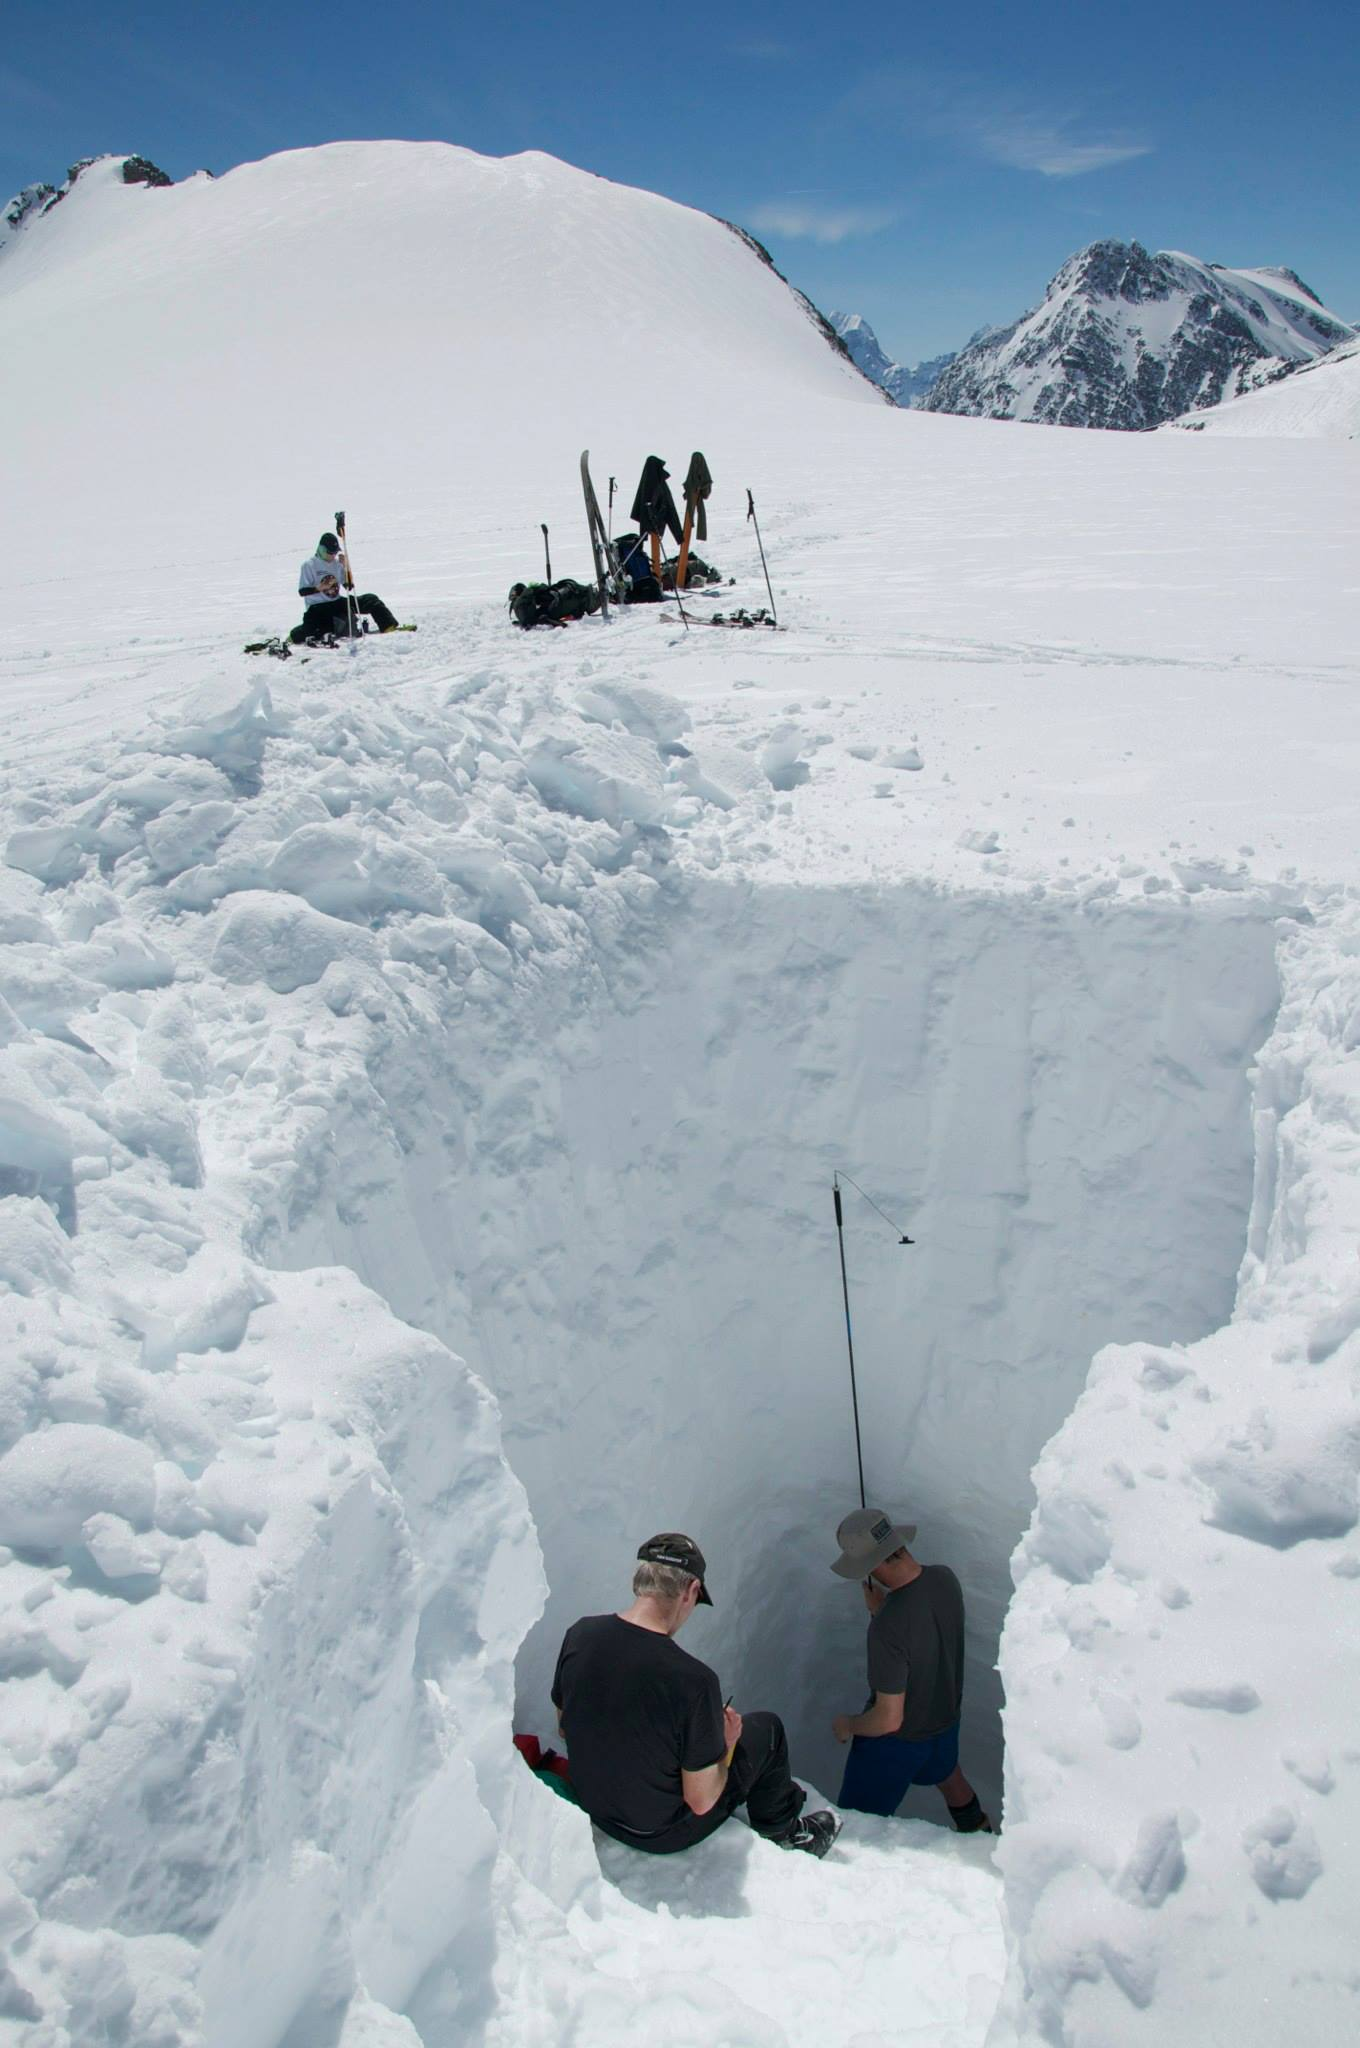
\includegraphics[width=0.5\textwidth]{snowpit.jpg}
  \caption{Digging a snowpit in the accumulation area of Haig Glacier, Rocky Mountains}
	\label{snowpit}
\end{wrapfigure}

The most direct way of measuring snow depth is by probing. To determine the snowpack thickness, the height of the snow above the end of the previous years ablation surface is measured. Usually, a number of snow height measurements are obtained close to each other and the mean value is taken to be representative of that location. For example, \cite{Machguth2006} took the mean of nine snow probes within a 7 m radius as representative of a test site in the ablation zone.  

In the ablation zone snow depth is easy to measure because the snow surface at the end of the melt season is well defined \citep{McGrath2015}. In the accumulation zone however, this same snow surface is determined by a combination of snow transformations --- including melt, settling, and redistribution by wind --- that are influenced by meteorological and topographical factors \citep{Grunewald2010}. This results in a heterogeneous snow surface that can have dense or compacted snow, ice lenses, or exposed firn. Furthermore, altering of the snow pack during the accumulation season (especially in the early and late parts) from warm weather or rain events can result in water refreezing in the snowpack \citep{Sold2014}. Probing in the accumulation zone can therefore result in erroneous depth measurements --- penetration into the dense snow or firn will make it seem like a deeper snowpack exists and probing to an ice lens within the snowpack can make it seem like shallower snow is present \citep{Sold2013}. As a result, snow pits and firn cores are often used to examine snow and firn layers to determine where the current season's snow begins.

To determine the glacier-wide SWE, point snow depth measurements from probing need to be extrapolated. This is often done using a statistical regression that accounts for grid cell values of slope, aspect, curvature, and susceptibility to wind redistribution \citep[e.g.][]{Wheler2014,McGrath2015}. This generates a linear equation that is site specific and is able to predict SWE for each grid cell based on the values of its relevant parameters. 

Snow probing is the simplest and oldest method used to determine accumulation. At the most basic level, it requires little more than a probe to determine depth, a way to determine location (such as a hand-held GPS), and a shovel to dig snow pits (see Figure \ref{snowpit}). Furthermore, this method directly measures snow depth so no data processing or corrections are needed and depth uncertainty is simple to quantify (often multiple depth measurements are taken close together) \citep{Sold2013}. 

There are however many drawbacks to this method. \textit{In situ} probing and digging snow pits are incredibly time-consuming \citep{Deems2006}. This limits the number of measurements that can be taken, which means that accumulation measurements are under-represented and spatial variability in accumulation is difficult to capture \citep{Sold2014}. Measurement is also limited to areas that are both accessible and safe for researchers. This means that in complex terrain many areas cannot be surveyed, resulting in data gaps. \citep{Sold2013} noted that this systematic bias can result in incorrect values of glacier-wide accumulation --- particularly because inaccessible areas such as cliffs and ridges have relatively shallow accumulations (due to wind erosion), while heavily crevassed areas can accumulate deep snow packs. 

\subsection{GPR}
\begin{wrapfigure}{L}{0.5\textwidth}
 \centering
      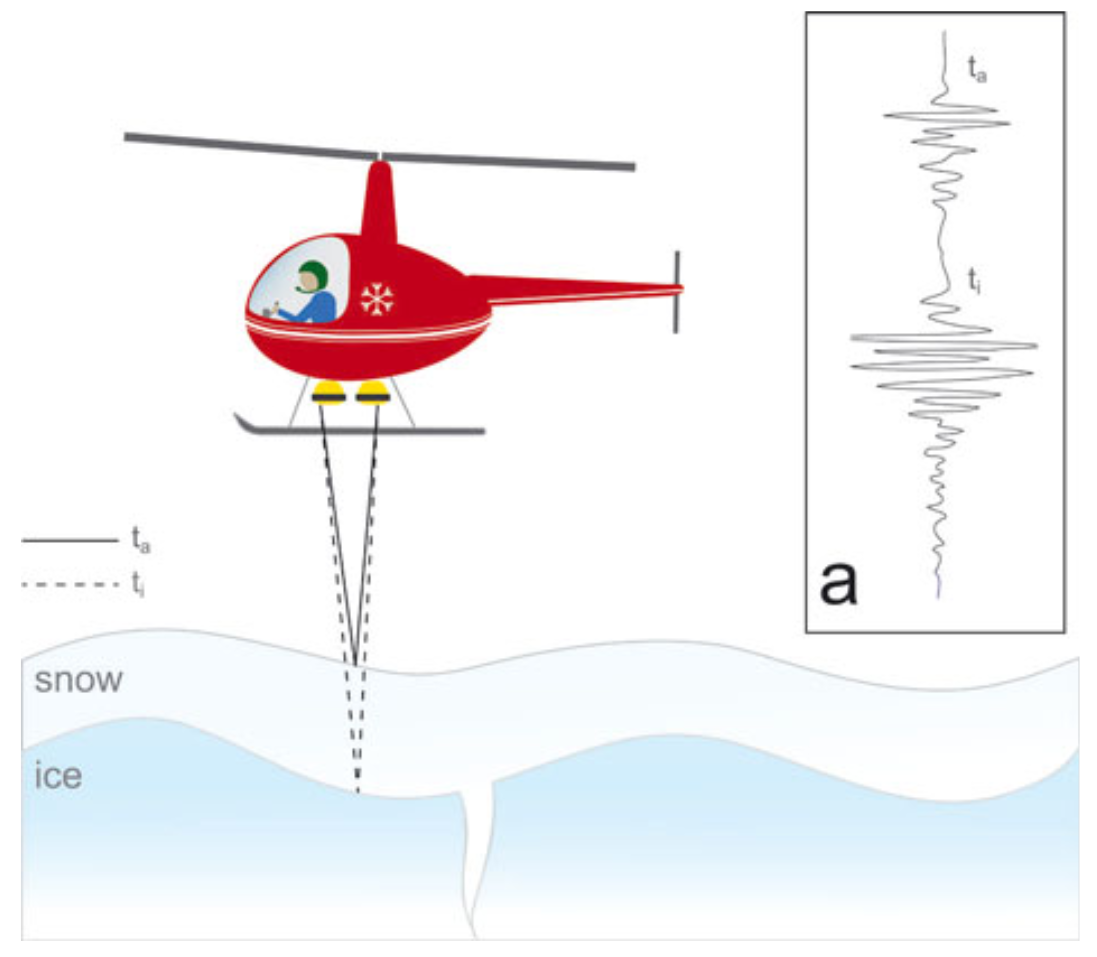
\includegraphics[width=0.5\textwidth]{gpr_air.png}
  \caption{Schematic of a helicopter-bore radar snow survey. The travel time for the signal to interact with the snow surface is snow as a solid line and the signal travel time of the interaction with the ice is shown as a dashed line. Together, these values can be used to determine snow depth. The inset (a) is an example waveform that would be recorded from these two events. Figure taken from \cite{Gusmeroli2014}.}
	\label{gprair}
\end{wrapfigure}

Ground penetrating radar (GPR) can be used to find snow depth along continuous lines. This method is used to calculate the distance from the radar source to a boundary with a strong contrast in dielectric permittivity, which corresponds to a change in material properties \citep{Sold2013}. When the speed of the radar wave through the material is known, the travel time can be measured and from this the distance calculated. On a glacier, the radar wave is able to penetrate snow and ice at MHz frequencies and the strongest reflections arise when water is present \citep{Sold2013}. To measure snow depth, GPR units are mounted on aircrafts or snowmobiles that then travel over snow covered areas (see Figure \ref{gprair})\citep{Machguth2006, McGrath2015}. The resulting radargram (e.g. Figure \ref{gpr}) gives a continuous snow depth profile. Processing of the radargrams involves using tracking algorithms that are able to trace continuous layers. Interpolation between transects is then done to find the glacier-wide accumulation. \cite{McGrath2015} describes this process in five steps: (i) acquisition of GPR and probing data (ground trotting), (ii) calculation of snow density and radar velocity, (iii) calculation of snow thickness and resulting SWE, (iv) applying a correction to measured accumulation based on ground truth data, and (v) using a multiple regression model to extrapolate SWE across the glacier. The extrapolation of SWE can also be done using an inverse approach with a coupled surface energy-balance snow model \citep{Pelt2014}.

GPR is an effective tool for measuring accumulation. It provides continuous snow depth transects, which means that spatial variability is well represented along the radar lines. GPR also has the major advantage that processes that affect snow height, including melt, settling, and glacier dynamics, do not affect the measurement accuracy \citep{Machguth2006}. Furthermore, the ability to fly over steep or inaccessible regions means that all areas of a glacier can be measured. GPR surveys also need be conducted only once to gain depth observations, which makes data collection fast and able to cover large areas \citep{Machguth2006}. 

A large limitation of GPR is the difficultly of processing radargrams. Areas where the snow-ice boundary is not well defined (i.e. the accumulation area) lack clearly contrasted material properties, which can lead to misinterpretation of their internal layers \citep{McGrath2015}. In the ablation area, the presence of crevasses can also result in radargram mislabeling \citep{Machguth2006}. Variation and uncertainty in radar wave speed due to differing snow density and liquid water content can also affect depth calculations \citep{Sold2013}. Often, wave speed is only measured in a few reference locations so changes in snow pack properties cannot be accounted for. Lastly, there is no universal procedure for processing GPR data. Selection of parameters and processing algorithms is dependent on field conditions, survey design and intention \citep{Sold2013}, which hampers the reproducibility of surveys.

\begin{figure}
 \centering
      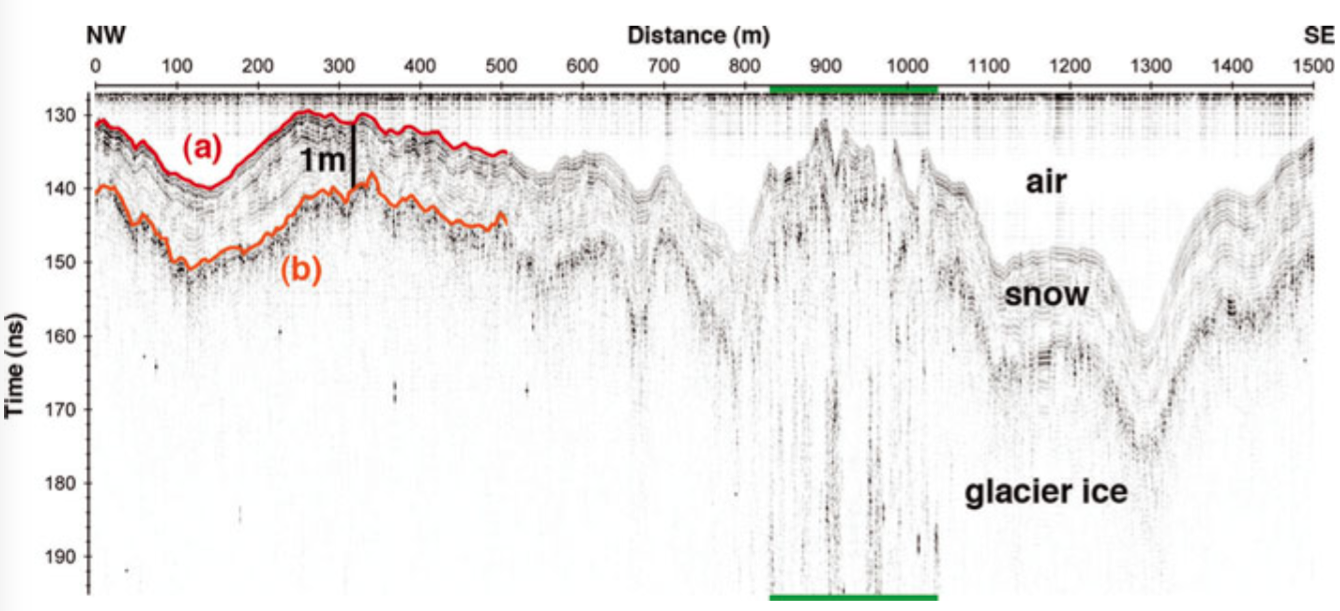
\includegraphics[width=\textwidth]{gpr.png}
  \caption{Radargram from the accumulation area of Findelengletscher, Valais, Switzerland. (a) The reflection at the air-snow interface. (b) The reflection at the snow-ice interface. Figure taken from \cite{Sold2013}.}
	\label{gpr}
\end{figure}

\subsection{DEM subtraction}
\begin{wrapfigure}{R}{0.5\textwidth}
 \centering
      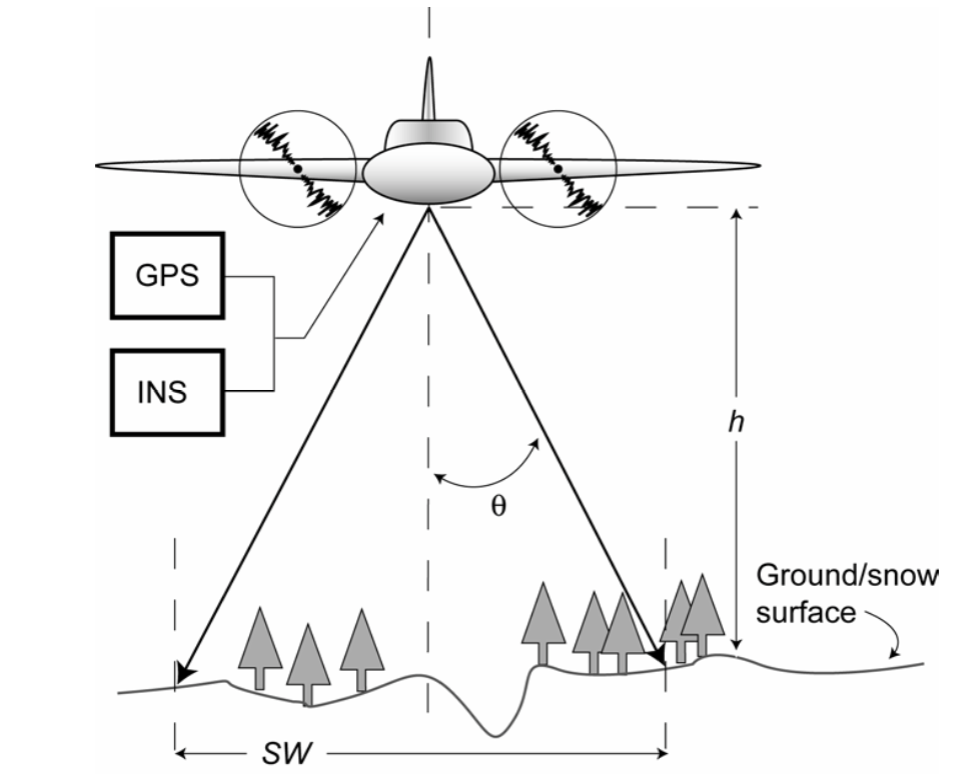
\includegraphics[width=0.5\textwidth]{lidar.png}
  \caption{Schematic of airborne LiDAR system geometry. Scan angle ($\theta$), height ($h$), and swath width ($SW$) are shown. Figure from \cite{Deems2006}.}
	\label{lidar}
\end{wrapfigure}
Digital elevation model (DEM) subtraction involves taking two detailed surface profile scans --- one at the end of the melt season and one at the end of the accumulation season --- and subtracting them from each other to find the snowpack height. The largest advantage of this remote sensing method is that it provides a highly resolved spatial measurement of snow depth over an entire basin \citep{Deems2006, Sold2013}. Data collection is fast, although two surveys must be conducted. This technique is sensitive to other processes that change the glacier surface elevation, including vertical displacement due to ice flow (positive in the ablation area and negative in the accumulation area), firn compaction, and surface lowering due to melt after the acquisition of the end of melt season DEM \citep{Sold2013}. For example, \citep{Sold2013} found that a first-order approach (where the observed elevation change was interpreted as snow accumulation) was inconsistent with snow depth probing --- DEM subtraction showed decreasing accumulation with an increase in elevation. Corrections can be made to account for these discrepancies but they rely on \textit{in situ} measurement of snow depth, knowledge of long-term mass balance, or information about the vertical displacement of ice from GPS towers \citep{Sold2013}. 

Lidar and photogrammetry are the two main methods of producing DEMs. Lidar produces a surface elevation model by calculating the distance to a target (by measuring the time between an emitted and return laser signal) \citep{Deems2006, Sold2013}. Terrestrial lidar systems involve stationary units placed in vantage points from which they are able to scan the basin surface \citep{Grunewald2010}. Large basins require multiple overlapping scans to acquire a complete surface profile. Airborne lidar systems (see Figure \ref{lidar}) can also only scan a certain size footprint so the aircraft must fly over all parts of the basin to acquire a full surface profile. These systems also require an accurate global positioning system (GPS) --- which is often corrected by referencing to a stationary GPS --- to determine the 3D locations of the surface \citep{Deems2006}. Airborne systems are widely applied and favourable in large basins or ones where no vantage point exists or is inaccessible. However, these systems are expensive so terrestrial scanners, which are comparatively more cost effective, are becoming popular \citep{Grunewald2010}. 

Complex topography and multiple laser reflections can cause problems when producing a DEM from lidar data \citep{Deems2006}. Significant vertical changes result in the spreading of the laser footprint and an incorrect interpretation of distance. \citep{Deems2006} shows that an error of 50 cm can result from lidar scans of 45$^\circ$ terrain from 1000 m flight height. Careful planning of flight paths can reduce this error. Scattering of laser light and penetration into the snow pack can also introduce error into height calculations, although its magnitude is small ($\sim$cm) \citep{Deems2006}. When subtracting the two measured DEMs, misclassification of corresponding point locations can occur, resulting in error in the final accumulation value \citep{Deems2006}.  

Photogrammetry uses photographs to produce a series of DEMs that can be subtracted to find snow depth. Early attempts in the 1960s at applying this technique in snow covered areas suffered from poor vertical resolution due to overexposed photographs and the necessity of manual differencing \citep{Nolan2015}. Modern photography equipment, GPS, and software technology have allowed for an increase in accuracy and lowering of costs associated with photogrammetry \citep{Nolan2015}. Current photogrammetry software is able to determine a snow surface profile relative to stable, snow-free points within the mapped area \citep{Farinotti2010}. The photos collected for DEM creation can also be used to identify suspect changes in the snow pack \citep{Nolan2015}.

Errors in photogrammetric measurements arise from sensor noise and poor lighting. Camera sensor noise is present in all digital photographs and its location changes from picture to picture. These erroneous pixels can be misinterpreted by the software as actual differences in height and thus lead to significant topographic noise, especially in steep mountainous terrain \citep{Nolan2015}. Additionally, having sufficient contrast in the photographed snow surface is critical for determining surface profile. Flat light conditions can reduce the resolution of the DEM or result in an absence of data in those parts of the photograph \citep{Nolan2015}. These effects can be avoided by waiting for better lighting. 

\subsection{Comparison of methods}
\label{sec:comparemethods}
The three methods of measuring accumulation differ in the extent of spatial information, collection techniques and costs, and processing needs. Spatial resolution is lowest for probing, which means that data must be interpolated. Although the actual measurement is simple and has low uncertainty, the interpolation of points can lead to misrepresentation of spatial variability and significant errors that are not quantified. GPR provides continuous snow depth profiles, but interpolation is still needed between lines. Further, significant errors can arise from interpretation of layers in radargrams. DEM differencing has the advantage of allowing for the measurement of surface profile across the whole basin, but error can result when glacier dynamics affect surface height changes. 

Large differences in data collection time and cost also exist. Probing has low equipment costs but requires a large amount of human hours for ground-based measurements. GPR and DEM subtraction both require the use of aircrafts and expensive electronic equipment. However, these methods have low human hour requirements and data collection occurs quickly.  

The three methods also have different data processing requirements. Simple statistical relations can be used for interpolating accumulation found by probing. However, GPR and DEM subtraction both require specialized software and knowledge of image processing methods, which increases the likelihood that misinterpretations of observations will occur. GPR has an advantage over DEM subtraction because it is not subject to elevation changes due to glacier dynamics and firn compaction. However, DEM subtraction has the advantage of more easily detecting the previous year's surface in the accumulation area \citep{Sold2013}. 

In general, \cite{Machguth2006} and \cite{Sold2013} found good correlations between probing measurements, GPR, and DEM subtraction. However, \citep{Sold2013} found that the methods did not always corroborate each other, particularly in crevassed areas and marginal regions. In crevassed areas, accumulation has large variation on small scales. The footprint of the GPR was usually too large to detect changes in snow depth and the movement of crevasses with time affected the lidar-derived snow depth. Marginal regions were misrepresented in the probing-derived profile because measurement was often not conducted in these areas (Section \ref{snowprobing}). This area also included the uppermost part of the glacier where wind erosion had a significant effect on accumulation. 

Choice of measurement technique for a snow survey is therefore dependent on project specific needs. Resolution, cost, and equipment availability need to be considered when selecting the most appropriate method. To reduce errors and misrepresentation of measurements, multiple methods can also be applied \citep{Machguth2006}. 

\subsection{Temporally resolved methods}
Temporally resolved methods measure accumulation continuously to provide a time series of snow accumulation. Usually, these methods involve relatively sparse point measurements so they do not represent spatial variability well. However, they are especially useful for identifying large snowfall events (rapid increases in accumulation) and wind erosion (gradual decreases in accumulation). 

There are a number of methods of measuring SWE with time. Snow depth sensors, such as the SR50, measure the time between emission and return of an ultrasonic pulse \citep{Ryan2008}. As snow accumulates, the distance between the sensor and the snow surface decreases. SWE is then calculated using an assigned density. Snow pillows, which are large (3 m diameter) bladders filled with antifreeze solution, directly measure SWE \citep{Archer1995}. As snow accumulates on the pillow, the weight of the snow forces an equivalent amount of the solution from the pillow to a standpipe. The height of the solution in the pipe is then recorded. Another method for measuring snow depth involves using multipath modulation of GPS signals \citep{Larson2009,McCreight2014}. Multipath modulation involves isolating GPS signals that are reflected from horizonal, planar reflectors, such as a snow surface. The distance between the geodetic GPS receivers and the reflection point will change during the accumulation season, thus recording changes in snow depth. This method allows for the measurement of average snow depth in a $\sim$1000 m$^2$ area around the antenna and an assigned density is then used to find SWE \citep{McCreight2014}.

\section{Snow distribution on glaciers}
While studies of snow distribution in alpine regions are plentiful \citep[and sources within]{Clark2011} there are comparatively few studies on the distribution of snow on glaciers. Although glaciers are often found in alpine environments, they present a different setting for accumulation. The freezing temperatures of glacier ice allow for snow to stick earlier than on the surrounding rocks, which can be above freezing especially in the early part of the accumulation season. Additionally, the surface of a glacier is often less steep than the surrounding peaks, which allows for snow to deposit more easily. The margin of the glacier can also accumulate snow from avalanches released from the surrounding peaks \citep{Bloschl1991, Mott2008}. Further, glaciers do not support vegetation, which has significant effects on snow accumulation in many alpine basins \citep{Pomeroy1999}. Since few studies have been done on this topic, it is difficult to say whether snow distribution on glaciers is fundamentally different than that of an alpine basin. This lack of snow variability quantification points to a significant gap in the literature.

\cite{Winther1998} conducted one of the first accumulation variability studies on a glacier. A GPR system was used to measure snow depth along three large transects on Spitsbergen, Svalbard. It was found that the accumulation-elevation gradients varied considerably and that regional variability was large, with almost 50$\%$ more accumulation on the eastern coast and a minimum in accumulation in the inland locations. A number of subsequent accumulation studies in Svalbard have since been conducted. \cite{Palli2002} used GPR along longitudinal profiles of Nordenskj\"{o}ldbreen and found 40-60$\%$ spatial variability over short distances. \cite{Grabiec2011} compared snow distribution on four types of glaciers in Svalbard. It was observed that the land-terminating mountain glacier had a simple altitudinal gradient while the outlet glacier had a much weaker correlation and more wind-redistributed snow. It was thought that the orientation and shape of the glacier also had a significant impact on snow accumulation, with the glaciers that were oriented parallel to the dominant wind direction having stronger altitudinal gradients. Another glacier that was observed had no altitudinal gradient, so its distribution was determined by complex local conditions. The ice cap that \cite{Grabiec2011} studied had all of these types of distributions in different areas.

\cite{Machguth2006} conducted an airborne GRP survey of two adjacent glaciers in Switzerland. The lower part of the larger valley glacier showed a clear correlation between altitude and snow accumulation. The upper part of the glacier and the adjacent smaller glacier had no altitudinal trend and the fluctuations in depth were large. Additionally, the accumulation was 40$\%$ lower on the smaller glacier. The altitudinal trend is a well documented pattern and was thought to be a result of melt that occurred during warmer weather, which is more pronounced at lower elevations. Spatial variability of precipitation and redistribution of snow were believed to have resulted in the high spatial variability in higher parts of the study area. Since the majority of the precipitation events originated from one direction and the large glacier was on the lee side of a ridge, it experienced preferential deposition. Meanwhile, the smaller glacier was further along the storm track so it received less precipitation. Overall, \cite{Machguth2006} showed that snow distribution on glaciers is not simply a function of altitude, which corroborated research done in other alpine catchments.

The most recent and comprehensive study of snow distribution on glaciers was done by \cite{McGrath2015}. This study focused on seven Alaskan glaciers of various sizes, orientations, and distances from the Pacific Ocean. \cite{McGrath2015} found that SWE was highly variable (40$\%$ differences) on hillslope scales and especially large in the ablation area (which has a rough surface due to the presence of crevasses). The dominant control on SWE distribution was altitude, but multiple terrain parameters were needed to capture most of the variance --- after elevation, wind exposure explained the most variance. 

The majority of studies that have examined snow distribution on glacier have been done with either airborne or ground-based GPR \citep[e.g.][]{Winther1998,Machguth2006, Grabiec2011, Pelt2014,McGrath2015}. In general, the radargrams provided valuable information but ground truthing by probing was always conducted. \cite{Gusmeroli2014} also did a small GPR survey on an Alaskan glacier and found that GPR reflections were difficult to identify in areas of the glacier that had high debris content on the surface or in the upper part of the accumulation area. \cite{Sold2013} did an extensive study that compared snow distribution values obtained by using probing, GPR, and DEM subtracting with lidar. All three methods showed an overall altitudinal trend but with significant small-scale variability (for a comparison of the three methods and their relative benefits, see Section \ref{sec:comparemethods}). \cite{Pelt2014} used GPR and a coupled surface energy balance-snow model to examine accumulation variability. It was found that the terrain parameters such as slope and curvature resulted in preferential deposition. Additionally, \cite{Pelt2014} calculated that small-scale variability of snow accumulation had a negligible effect on the mean net mass balance in the accumulation zone and a negative impact of -0.09 m w.e. a$^{-1}$ in the ablation area.

\cite{Dadic2010} is the only study thus far that has examined snow distribution on glaciers using a dynamic model. This study specifically looked at the effect of wind on snow accumulation, and found that glacierized areas with the largest accumulation also experienced the slowest horizontal wind speeds and increasing downward wind velocity. Preferential deposition was highest (positive or negative) in troughs located close to steep slopes, where updrafts and down drafts led to decreased and enhanced deposition, respectively. In general, the wind speed was controlled by small-scale topography and had a significant impact on accumulation. 

Although there are still few studies of snow distribution on glaciers, the work described above provides a good starting point for such investigations. Comparisons of variability between neighbouring glaciers and within a basin are both important areas of study.

\section{Glaciers in the St. Elias Mountains}
\begin{figure}
 \centering
      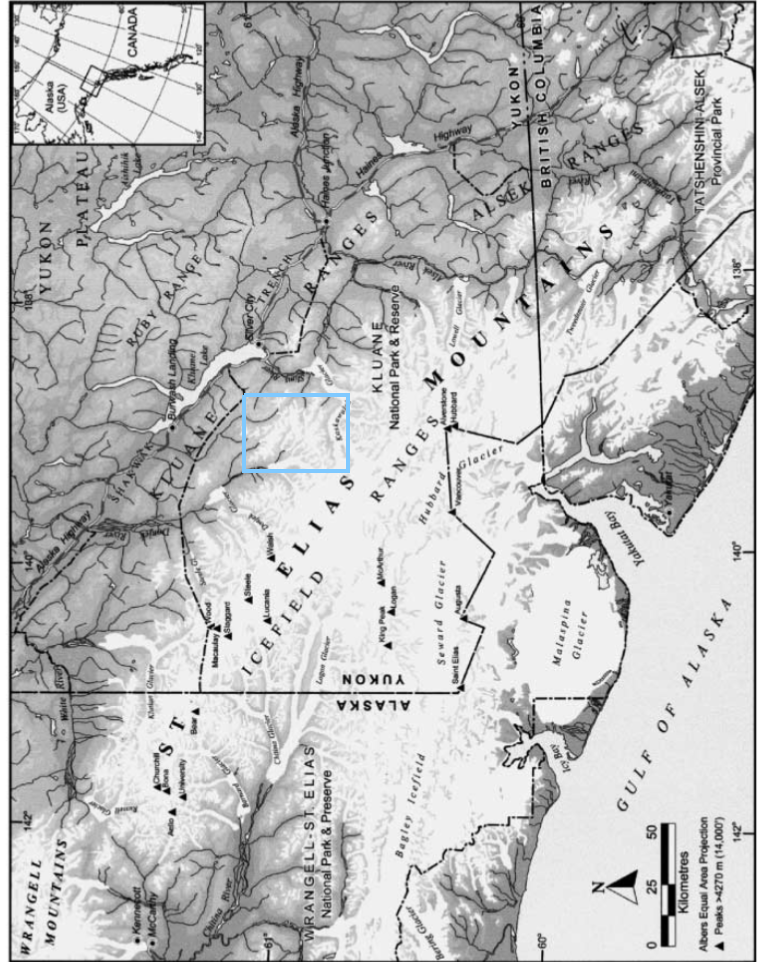
\includegraphics[width=\textwidth]{stelias.png}
  \caption{Map of the St. Elias Mountains and surrounding area. Figure taken from \cite{Danby2003}.}
	\label{map}
\end{figure}

Snow data are generally sparse in mountain regions, especially those that are isolated from humans \citep{Marcus1970}. The St. Elias Mountains (Figure \ref{map}) are one such area. These mountains contain the largest non-polar ice field and the longest valley glaciers outside of Greenland and Antarctica \citep{Marcus1970, Danby2003}. Steep climatic gradients across the mountains create sharp changes in glacier cover and mass balance \citep{Clarke2002}. This region currently has the most negative mass budget and is the largest contributor to sea-level rise in the world \citep{Kaser2006, Gardner2013}. Understanding how local glacier mass balance is affected by distribution of snow is therefore critical for accurate predictions of glacier response to a warming climate. 

Research on snow distribution and glacier mass balance in the St. Elias is limited. The first significant investigations took place under Project Snow Cornice \citep{Wood1948}. Researchers looked at snow accumulation and ice formation as well as ice-mass thermal regime, density, and depth. Studies were conducted primarily on large glaciers such as the Kaskalwalsh and Seward, and thus provided insights into large-scale accumulation patterns. This initiative was then followed by the Icefield Ranges Research Project (IRRP), which was established in 1961 \citep{Danby2003}. A number of subsequent long-term studies have been established in the St. Elias since IRRP. The mechanisms associated with surge type glaciers were studied by Garry Clarke and his colleagues on Trapridge Glacier \cite{Clarke1984}. More recently, Gwenn Flowers began studying smaller alpine glaciers in the eastern part of the St. Elias Mountains \citep[e.g.][]{Paoli2009}. \cite{Wheler2014} determined the end-of-winter accumulation for the mass balance of these glaciers by recording snow depth at a number of fixed stakes and using a multiple linear regression model --- that accounted for slope, curvature, and elevation --- to extrapolate these points and find SWE. \cite{Arendt2008} also briefly studied the mass balance of a number of glaciers in the St. Elias.

Two ice cores have been retrieved from the St. Elias Mountains. The first one was taken from the summit of Mt. Logan (5340 m) in 1980 and was 103 m long. The accumulation history in this core has been used to study the local \citep{Holdsworth1991} and regional \citep{Moore2002} climate history. A second core, called the Eclipse core, was taken from a site 45 km northeast of Mt. Logan, 2 km lower in altitude, with an accumulation almost five times as large \citep{Wake2002}. This core is 160 m and has also been used for studying local and regional climate history \citep{Wake2002}. 

The weather in the St. Elias varies considerably over the range. The west side of the mountains is characterized by a cool, Marine West Coast climate due to the influence of the Pacific ocean, while the eastern side (just 250 from the ocean) is considered subarctic \citep{Marcus1970}. \cite{Taylor1969} studied the relationship between synoptic weather conditions and basin weather conditions across the St. Elias. It was observed that the mountains are oriented perpendicular to frequent and intense storms that originate in the ocean, which resultes in considerable interaction between weather and topography. When weather moves from the Gulf of Alaska, it is orographically lifted, which creates significant precipitation. If the front is perpendicular to the mountains, it can be deflected north or south, depending on the upper atmospheric flow. Fronts that are more or less aligned parallel to the mountains or very strong perpendicular fronts travel without deflection. The fronts can also stall on the west side of the mountains. Eventually, the fronts spill over the mountain divide (located to the west of the Kaskawalsh Glacier) and descend along the eastern side, which often results in decreased precipitation. This rain shadow is likely the major cause of the significant difference in accumulation and equilibrium line altitude (ELA) between the two sides of the mountains --- the marine side has an ELA of $\sim$1100 m and the continental side has an ELA of $\sim$2100 m, while at the same elevation there is three times more accumulation on the marine side \citep{Marcus1970}.

Although the characterization of synoptic conditions by \cite{Taylor1969} is useful, it was conducted during the summer when weather conditions are considerably different than during winter. \cite{Taylor1969} does note though that the weather patterns observed would likely be strengthened during winter because many of the spatial gradients are enhanced. The synoptic air masses present during the winter produce a strong temperature and moisture gradient, with warm, moisture-laden air coming from the Pacific Ocean and cold, dry air coming from the Mackenzie basin. These gradients would likely result in even more precipitation and stronger winds. The presence of a high pressure Arctic system could decrease the ability of low-pressure systems to pass over the divide, leading to a further enhancement of precipitation on the western side of the mountains. 

The study done by \cite{Taylor1969} also found weather effects on multiple scales. Synoptic conditions, including front movement, affected regional scale differences in weather; watershed scale topography was responsible for differences in weather for nearby basins and affected wind speed and direction most significantly; and point scale topography had strong effects on snow accumulation. Orographic effects were found to be significant on all scales. 

A study done by \cite{Pomeroy1999} looked at snow mass balance in a non-glacierized alpine basin within the St. Elias. It was found that wind had a significant impact on the distribution of snow --- up to 79$\%$ of the snow was redistributed from alpine areas to (primarily) hillsides, where accumulation was tripled. In the study basin, measured accumulation ranged from 54$\%$ to 419$\%$ of the actual snowfall. However, in a subsequent study year, which had two large wet snow events, the redistribution of snow was minimal and accumulation variability was much lower. The type of snow and how susceptible it is to wind effects therefore also plays a critical role in distribution. Additionally, areas within the basin can have different accumulation patterns throughout the winter. One area within the basin studied by \cite{Pomeroy1999} had almost no redistribution (despite heavy winds) from the beginning of winter through to March. After this, all of the snow was lost even though additional accumulation events occurred in the basin. This could indicate a dependence of redistribution on weather conditions such as temperature, or that a critical depth was reached that allowed for redistribution to occur. Sublimation was also observed in the basin, but the amount of snow lost through this process could not be determined. Yet given that sublimation occurs several orders of magnitude faster when blowing snow is present and approximately 20$\%$ of winter days were observed to have blowing snow, it could have a significant impact.

There is clearly a strong need for a more comprehensive understanding of snow accumulation in the St. Elias Mountains. Although a few studies have examined accumulation, no studies have examined the distribution of snow and how it varies spatially. This is especially true of small alpine glaciers in the St. Elias Mountains, since the majority of accumulation differences have been observed on large glaciers. It is likely that orographic lifting as well as wind redistribution and preferential deposition play major roles in determining accumulation on small alpine glaciers, so future studies should focus on the impact of these factors. 

\section{Summary}
Snow accumulation plays a central role in alpine hydrology and has a prominent impact on glacier mass balance. In mountainous regions, accumulation is highly variable on point, hillslope, watershed, and regional scales. This is due to complex interactions between dynamic meteorology and dramatic topography that result in steep gradients in temperature and wind. Processes such as orographic lifting, preferential deposition, and wind redistribution are a result of these interactions and they affect where snow will accumulate. 

The distribution of snow can be described using dynamic and statistical models. Dynamic models employ equations that describe physical processes to determine local atmospheric conditions and from that, calculate where snow is likely to accumulate. These models are spatially and temporally transferable and provide insight into relevant processes. However, they are computationally expensive and require a large array of input data. Statistical models, on the other hand, are computationally simple and usually require only basic data. However, their use is restricted to areas with long historical records, and their transferability limited by the fact that the parameters they employ are proxies for processes.

Measuring snow accumulation can be done a number of different ways. Snow probing is the simplest method and requires little equipment and knowledge. However, the measurements acquired are usually quite sparse, require a long time to complete, and cannot be done in areas that are difficult to access. GPR is another common way of measuring snow depth and has been widely applied in snow accumulation studies. This technique provides continuous lines of snow depth data and is not affected by surface changes due to glacier dynamics. Processing and interpreting data can be difficult though, especially in the accumulation area. DEM subtraction allows for a fully distributed measurement of accumulation but complex topography can create significant errors in the interpretation of distance. Factors such as cost, processing needs, and extent of spatial information should all be considered when determining which method to apply.

Snow accumulation on glaciers is a relatively new area of research. The few studies that have examined this topic have found high variability in accumulation both within a glacierized basin and between nearby glaciers. Perhaps the most challenging aspect of studying accumulation on glaciers is acquiring data with sufficient spatial extent and resolution to come to meaningful conclusions. Determining processes relevant to snow distribution also presents considerable difficultly since dynamic models are sparse and statistical models must employ proxy parameters. In the St. Elias Mountains, little is known about the variability of snow distribution on alpine glaciers. No studies have been done to examine differences in accumulation between glaciers within the same range and accumulation distribution within those glaciers. Given the importance of snow for local water availability and glacier mass balance, there is clearly a need to better understand its distribution within the St. Elias Mountains.


\bibliography{MastersLit}
\bibliographystyle{igs}
\end{document}
